% !TeX encoding = UTF-8
% !TeX program = xelatex
% ----------------------------------------------------------------------------------------------------------------
% Appel des packages de base
% ----------------------------------------------------------------------------------------------------------------
\documentclass[10pt,a4paper]{report}
\usepackage{styles/preambule_college}
\usepackage{styles/preambule_personnalisation}


\setcounter{secnumdepth}{3}



%\definecolor{darkblue}{rgb}{0.12,0.47,0.87}
%
%\titleformat{\chapter}[display] 
%	{\fontsize{17pt}{12pt}\selectfont \bfseries}
%	{\textcolor{darkblue}{\chaptertitlename\ \thechapter: #1}}
%	{20pt}
%	{\Huge}
%
%\titleformat{name=\chapter,numberless}[display] 
%	{\fontsize{17pt}{12pt}\selectfont \bfseries}
%	{\textcolor{darkblue}{#1}}
%	{20pt}
%	{\Huge}

% ----------------------------------------------------------------------------------------------------------------
% Début du document
% ----------------------------------------------------------------------------------------------------------------
\begin{document}





\chapterFormat




\chapter*{Environnement de travail}

Le collège met à disposition des étudiants et des professeurs divers outils informatiques. Pour être efficient dans son travail, il est nécessaire d'en connaître l'existence et l'usage\dots





\section{Infrastructure du collège}



\subsection{Machines et réseau}

Des \emphdef{ordinateurs fixes} sont à disposition à la bibliothèque, dans les salles de classe et dans les salles informatiques.

Les photocopieurs peuvent être utilisés comme \emphdef{imprimante} : 
\begin{enumerate}
	\item Depuis les postes fixes, il faut choisir \emph{LCC Printer} dans la liste des imprimantes. Lorsqu'on lance l'impression, le document ne sort pas physiquement d'un photocopieur, mais il est placé dans un \emph{serveur d'impression}. Pour récupérer ses copies, il faut s'identifier sur un photocopieur à l'aide de sa carte du LCC et choisir le document à imprimer dans la liste. Le document ne s'imprime que si le montant disponible sur la carte est suffisant.
	\item Depuis une clé USB, les photocopieurs peuvent lire un document photo ou PDF directement depuis une clé USB. Pour cela, elle doit être \emphdef{formatée} en FAT.
\end{enumerate} 

Les photocopieurs peuvent \emphdef{scanner} des documents. Le photocopieur crée alors un document PDF qui peut être enregistré sur une clé USB ou envoyé par mail à l'adresse de son choix.

Le \emphdef{WiFi} est disponible dans tout l'établissement. Évidemment, vu le nombre d'étudiants qui peuvent être présents simultanément dans les parties communes (hall, cafétéria\dots) et les limitations intrinsèques du WiFi, il ne faut pas s'attendre à des miracles à ces endroits durant les pauses\dots

\attention Ces infrastructures sont dédiées au travail. Cela veut dire que tout ce qui passe sur le réseau fait l'objet d'une surveillance. Cela permet à l'établissement de déterminer au besoin qui a utilisé l'infrastructure à mauvais escient et de prendre les mesures correspondantes.



\subsection{Identifiant}

Chaque étudiant ou professeur doit se connecter avec son identifiant (nom d'utilisateur et mot de passe) pour accéder à l'infrastructure informatique. Le nom d'utilisateur est public ou peut être deviné par n'importe qui. Le mot de passe est personnel et doit le rester.

\attention Toute activité effectuée par un utilisateur identifié sur le réseau est de la responsabilité de la personne qui a défini le mot de passe correspondant. C'est de la responsabilité de chaque utilisateur de changer de mot de passe aussi souvent que nécessaire.

\exemple*{
	Alice a eu accès au mot de passe de Bob, peut-être parce que Bob le lui a donné, ou parce qu'il l'avait écrit dans un endroit accessible. Peut-être aussi parce que le mot de passe était facile à deviner ou parce que Bob utilise tout le temps le même depuis des années ou encore parce qu'il n'en a qu'un seul pour différents services (ses comptes Instagram, Tik Tok, Snapchat\dots). Peut-être aussi Bob s'est-il montré naïf en remplissant un faux questionnaire l'incitant à changer son mot de passe ou en répondant à un faux appel téléphonique\footnote{Il s'agit de \emphdef{phishing} appelé aussi \emphdef{hameçonnage}.}\dots \ Dans tous les cas, Alice peut se connecter à l'infrastructure en se faisant passer pour Bob, faire ce qu'elle veut et ce sera à Bob d'assumer ce qu'elle fait !
}

\remarque*{
	Au passage, Alice a commis quelques infractions, non seulement par rapport au règlement du collège et à la charte informatique, mais aussi au regard du droit suisse. Le Code pénal ne punit pas encore l'usurpation d'identité en tant que telle, mais une modification de l'art. 179 devrait bientôt le permettre (voir \autocite{UsurpationIdentiteEstelle2021}). Dans tous les cas, selon ce qu'a fait Alice après s'être connectée, elle pourrait être accusée de s'être introduite sur un système informatique sans en avoir le droit (art. 143), d'avoir calomnié ou diffamé Bob, de l'avoir escroqué, d'avoir utilisé frauduleusement un ordinateur\dots \ Ce sont des infractions qui peuvent conduire à des amendes voire à de la prison.
}



\subsection{Services en ligne}

L'identifiant personnel donne accès non seulement aux machines du collège, mais aussi aux services en ligne suivants.



\subsubsection{\href{creusets.net}{creusets.net}}

Le site web du collège ne sert pas uniquement à télécharger la liste de classe lors de la dernière semaine des vacances ! Il permet de trouver toutes les informations pratiques et, uniquement pour les personnes connectées, d'accéder à des téléchargements particuliers ou à des galeries de photo.

\begin{figure}[H]
	\centering
	\href{https://creusets.net}{
		
\includegraphics[width=0.75\linewidth]{images/capture_creusets_20210811.png}
	}
	\caption{\protect \href{https://edu.vs.ch}{Site web du collège}}
	\label{fig:capturecreusets20210811}
\end{figure}

Le site est accessible à l'adresse \href{https://creusets.net}{https://creusets.net}.



\subsubsection{Plateforme d'apprentissage : \href{https://moodle-lcc.edu-ictvs.ch/}{Moodle}}

Moodle est un système de gestion de contenu ou \emphdef{Content Management System} (CMS) en anglais. Moodle est un CMS dédié à l'enseignement. Il s'agit d'un logiciel libre développé depuis une vingtaine d'années et utilisé par plusieurs centaines de milliers de sites Web dans plus de 200 pays. Toutes les grandes universités l'utilisent, en particulier en Suisse.

\begin{figure}[H]
	\centering
	\href{https://moodle-lcc.edu-ictvs.ch/}{
		
\includegraphics[width=.75\linewidth]{images/capture_moodle_lcc_20210811}
	}
	\caption{\protect\href{https://moodle-lcc.edu-ictvs.ch/}{Moodle LCC}}
	\label{fig:capturemoodlelcc20210811}
\end{figure}

Le Moodle LCC est accessible à l'adresse suivante : \href{https://moodle-lcc.edu-ictvs.ch/}{https://moodle-lcc.edu-ictvs.ch}

\encadre[Les logiciels libres]{
	Il existe plusieurs définitions d'un \emphdef{logiciel libre} (voir par exemple \autocite{LogicielLibre2021}). Toutes reprennent cependant les bases posées par la \href{https://www.gnu.org/philosophy/free-sw.html}{Free Software Foundation} (FSF). Ce type de logiciel garantit que "les utilisateurs ont la liberté d'exécuter, copier, distribuer, étudier, modifier et améliorer ces logiciels" \autocite{DefinitionLogicielLibre}. N'importe quel programmeur (vous dans quelques mois peut-être) peut donc voir comment est fait le logiciel pour en comprendre le fonctionnement détaillé. Cela peut servir à vérifier qu'il ne s'y cache rien de malveillant, de corriger des bugs ou de proposer de nouvelles fonctionnalités.\\[1ex]
	La plupart du temps, ces logiciels sont d'ailleurs gratuits, même si gratuité n'est pas synonyme de liberté. Selon la FSF :
	\enquote{\textelp{} “free software” is a matter of liberty, not price. To understand the concept, you should think of “free” as in “free speech,” not as in “free beer”.} \autocite{WhatFreeSoftware}.\\[1ex]
	La \emphdef{licence} d'un logiciel est ce qui détermine ce qu'on a le droit de faire avec. Les principales licences libres sont les \href{https://fr.wikipedia.org/wiki/Licence_publique_g\%C3\%A9n\%C3\%A9rale_GNU}{GNU} \autocite{LicencePubliqueGenerale2021}, \href{https://fr.wikipedia.org/wiki/Licence_BSD}{BSD} \autocite{LicenceBSD2021} ou \href{https://fr.wikipedia.org/wiki/Licence_Apache}{Apache} \autocite{LicenceApache2021}.
}



\subsubsection{\href{https://edu.vs.ch}{ENT}}

Le canton du Valais met à disposition une plateforme nommée ENT pour "environnement numérique de travail". Il s'agit d'un produit commercial de Microsoft.

\begin{figure}[H]
	\centering
	\href{https://edu.vs.ch}{
		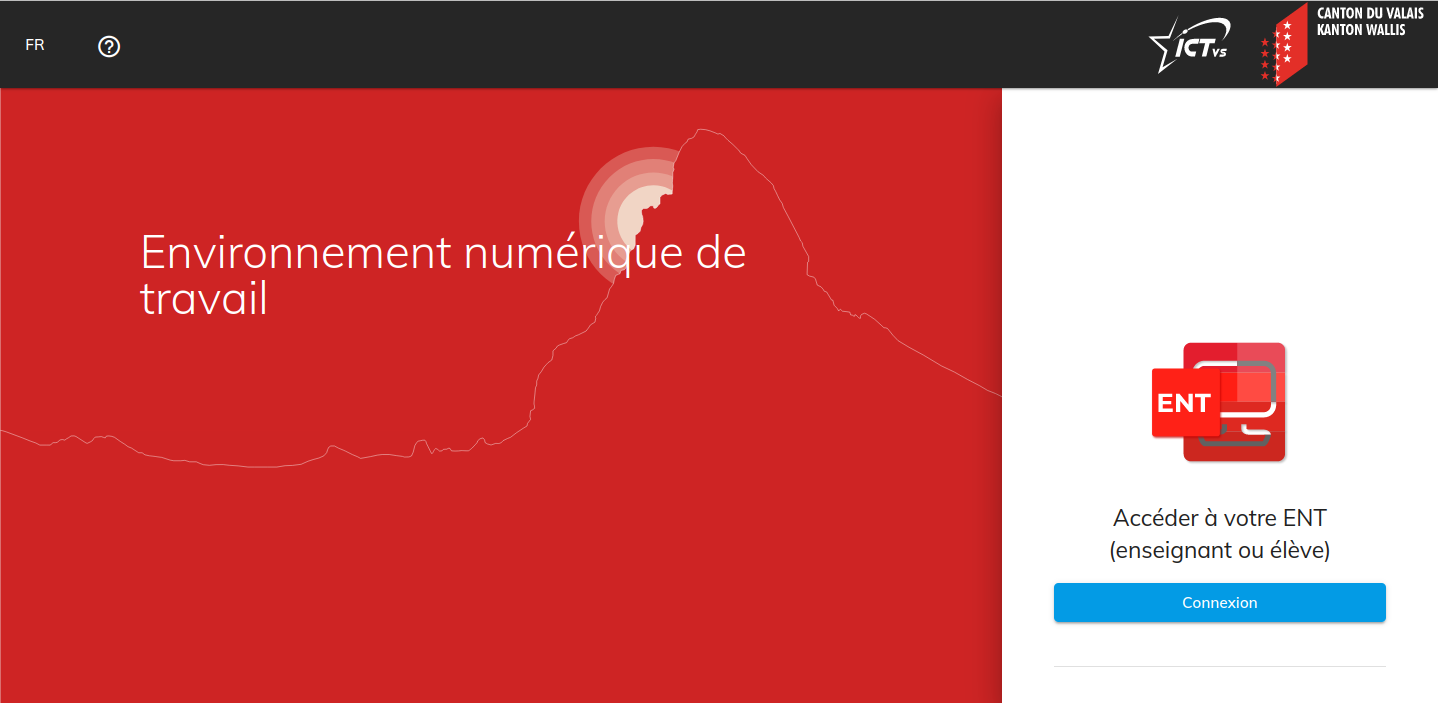
\includegraphics[width=0.75\linewidth]{images/capture_ENT_20210811.png}
	}
	\caption{\protect \href{https://edu.vs.ch}{ENT -- Environnement numérique de travail}}
	\label{fig:captureent20210811}
\end{figure}

L'accès à l'ENT se fait à l'adresse \href{https://edu.vs.ch}{https://edu.vs.ch}.

La page principale présente les divers produits sous forme de tuiles.

\begin{figure}[H]
	\centering
	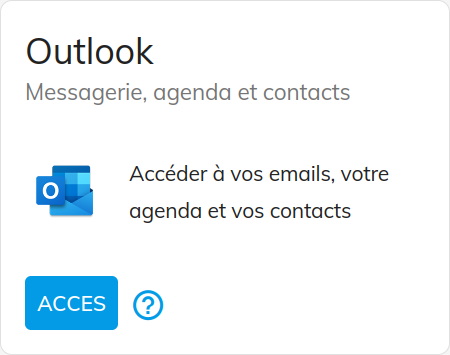
\includegraphics[width=0.18\linewidth]{images/capture_ENT_tuile_outlook_20210811}
	\hfill
	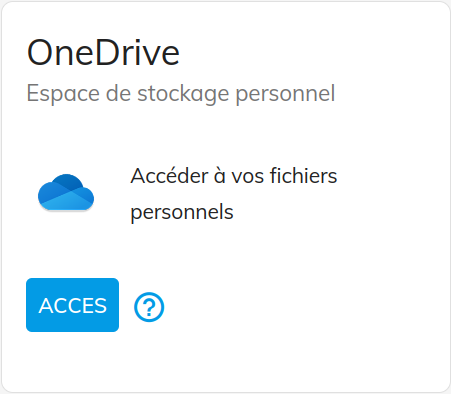
\includegraphics[width=0.18\linewidth]{images/capture_ENT_tuile_OneDrive_20210811}
	\hfill
	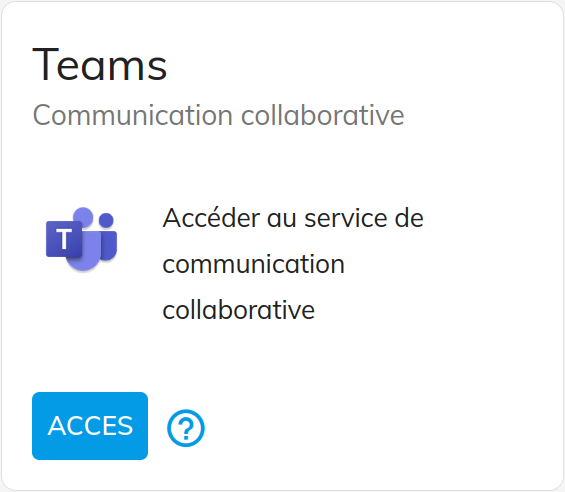
\includegraphics[width=0.18\linewidth]{images/capture_ENT_tuile_Teams_20210811}
	\hfill
	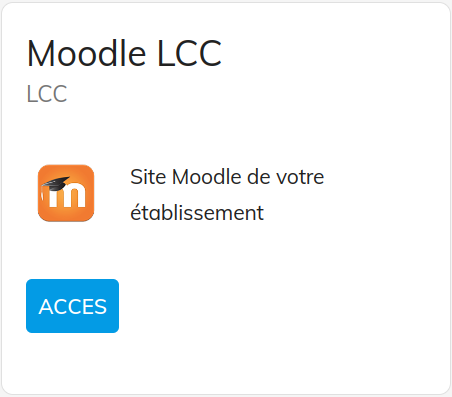
\includegraphics[width=0.18\linewidth]{images/capture_ENT_tuile_moodle_20210811}
	\caption{Tuiles des fonctions principales de l'ENT}
	\label{fig:tuilesENT}
\end{figure}

\begin{description}
	\item[Outlook] Ce terme regroupe différentes choses distinctes :
		\begin{itemize}
			\item un service d'e-mails avec les contacts et les agendas;
			\item des logiciels permettant de se connecter au service e-mail. Il en existe des versions pour téléphone mobile (sous Android ou iOS), pour ordinateurs Apple sous OS X et pour ordinateurs Windows;
			\item les serveurs sur lesquels se trouvent les e-mails;
			\item l'interface \emphdef{webmail} qui permet de se connecter aux serveurs depuis son navigateur. 
		\end{itemize}
		Il est possible d'accéder aux services de messagerie sans application Outlook, simplement depuis la tuile présente dans l'ENT. \\
		Il est aussi recommandé d'installer une application de messagerie sur son ordinateur et son téléphone pour accéder plus directement à ses e-mails. À noter que sur Android, Apple (iOS ou OS X), Windows ou Linux, il existe déjà des applications qui permettent de se connecter à son e-mail. Elles sont souvent préinstallées et il n'y a donc pas besoin de rajouter encore l'application Outlook à sa machine. Il suffit alors de rajouter son compte mail @eduv.vs.ch dans la liste des comptes gérés par l'application existante.
	\item[OneDrive] un espace de stockage pour y déposer et synchroniser ses fichiers.
	\item[Teams] Il s'agit d'un logiciel de visioconférence et de travail collaboratif. Pour faire une visioconférence, il faut évidemment que l'ordinateur dispose d'une caméra et d'un micro, ce qui n'est pas le cas des ordinateurs des salles de classe ni de la bibliothèque.
	\item[Moodle] Lien vers le Moodle LCC depuis l'ENT (voir ci-dessus).
\end{description}

\remarque*{
	Pour toute question concernant l'ENT, commencez par aller lire les informations sur \href{https://support.ictvs.ch/index.php/fr/}{https://support.ictvs.ch/index.php/fr/}
}

\encadre[Les logiciels propriétaires]{
	Les logiciels propriétaires sont le contraire des logiciels libres. La plupart des logiciels commerciaux sont de ce type. Ainsi, une entreprise garde le secret sur la manière dont est faite son logiciel. Comme utilisateur, on ne peut pas savoir ce qu'il fait réellement et encore moins le modifier. \\[1ex]
	Le \emphdef{reverse engineering} ou \emphdef{rétro-ingénierie} est un procédé permettant d'étudier un logiciel pour en comprendre le comportement lorsqu'on ne peut pas savoir comment il a été conçu. Cette pratique est illégale la plupart du temps\dots
}







\section{Bases de l'utilisation}



\subsection{Organiser ses fichiers}

Même si certaines fonctionnalités permettent de retrouver des fichiers sur son ordinateur, il vaut la peine de réfléchir à l'organisation de ses fichiers en répertoires et sous-répertoires. Cela simplifie grandement les recherches, évite les doublons, permet de sauvegarder et de restaurer facilement les documents\dots

Au collège, une bonne manière de commencer est de faire un répertoire par année et des sous-répertoires par branche.



\subsection{Traitement de texte}

Le traitement de texte est un outil qu'il est nécessaire de connaître pour faire des études. Plus vite vous vous y mettrez, mieux vous vous porterez. Il existe des versions libres et vraiment gratuites telles que LibreOffice, OpenOffice ou NeoOffice (sur Mac) et d'autres propriétaires et apparemment gratuites comme Office 365 (payée par le canton) ou Google Docs (Vous êtes le produit de Google\dots)

\remarque*{
	Lorsqu'on met en forme un texte de manière professionnelle, il est \emph{nécessaire} d'utiliser les \emphdef{styles}. \\
	Si vous ne le faites pas habituellement ou si vous ne savez pas ce que c'est, trouvez-vous un tutoriel le plus rapidement possible !
}



\subsection{Utilisation du mail}

Chaque membre de l'établissement a une adresse prenom.nom@edu.vs.ch. Il s'agit d'un moyen de communication professionnel et il convient de l'utiliser comme tel. En particulier, un e-mail correctement rédigé :
\begin{itemize}
	\item comporte l'adresse du destinataire (sans cela votre e-mail n'ira pas bien loin);
	\item le sujet qui précise le contenu du mail (ce champ est visible lorsque les e-mails sont présentés sous forme de liste et aide s'y retrouver);
	\item en début de courrier, une formule d'annonce avec les civilités (Madame, Monsieur\dots);
	\item à la fin du courrier, une formule de salutation (au minimum "Meilleures salutations");
	\item une signature (votre prénom, votre nom et votre classe).
\end{itemize}

Un e-mail professionnel doit être rédigé en utilisant un registre de langage soutenu et en évitant les familiarités, les abréviations et les émoticônes.



\subsection{Télécharger des documents}

Pour récupérer des documents depuis un navigateur web, il existe plusieurs options :

\begin{enumerate}
	\item On peut cliquer sur un lien et une fenêtre permet de choisir d'ouvrir ou de télécharger le document.
		\begin{figure}[H]
			\centering
			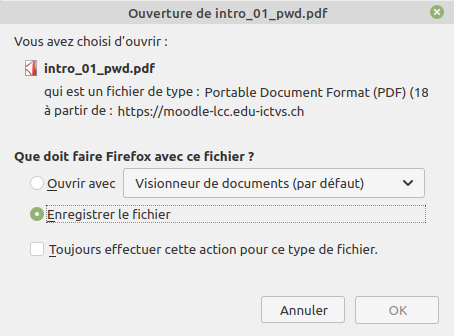
\includegraphics[height=4.5cm]{images/capture_telechargement_01}
			\caption{Télécharger un document}
			\label{fig:capture_telechargement_01}
		\end{figure}
		\attention Pour les documents du cours, il faut choisir de les télécharger. Ainsi on en dispose d'une copie sur sa machine, même lorsqu'on n'est pas connecté au réseau.
	\item Certains documents s'ouvrent directement dans le navigateur sans présenter la boîte de dialogue précédente. Ou parfois, on veut simplement récupérer une image sur un site web. Dans ce cas, on peut faire apparaître la boîte de dialogue en faisant un clic droit sur la page ou l'image et en choisissant \emph{Enregistrer sous\dots}, \emph{Sauvegarder sous\dots}, \emph{Enregistrer l'image sous\dots} ou équivalent dans le menu contextuel. \\
		\begin{minipage}{.4\linewidth}
			\begin{figure}[H]
				\centering
				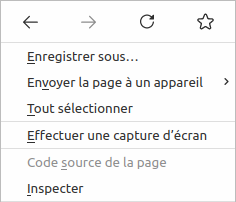
\includegraphics[height=3.5cm]{images/capture_telechargement_02}
				\caption{Enregistrer sous\dots}
				\label{fig:capture_telechargement_02}
			\end{figure}
		\end{minipage}
		\hfill
		\begin{minipage}{.45\linewidth}
			\begin{figure}[H]
				\centering
				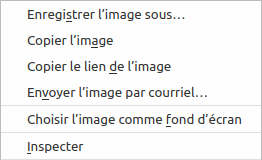
\includegraphics[height=2.75cm]{images/capture_telechargement_03}
				\caption{Enregistrer l'image sous\dots}
				\label{fig:capture_telechargement_03}
			\end{figure}
		\end{minipage} \\
	\item Dans certains cas il n'y a qu'un lien qui ne s'ouvre pas dans le navigateur. On peut essayer de faire un clic droit et de choisir l'option \emph{Enregistrer la cible du lien sous\dots} ou équivalent.
		\begin{figure}[H]
			\centering
			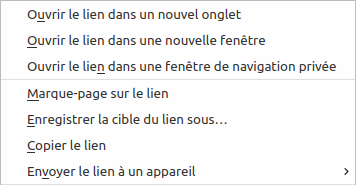
\includegraphics[height=3cm]{images/capture_telechargement_04}
			\caption{Enregistrer la cible du lien sous\dots}
			\label{fig:capture_telechargement_04}
		\end{figure}
\end{enumerate}

\attention Par défaut, les documents sont téléchargés dans un répertoire appelé \emph{Téléchargements}, \emph{Downloads} ou autres situés dans son répertoire principal. Il faut ensuite les déplacer dans le répertoire de son choix. Ce n'est généralement pas une bonne idée de laisser tous ses téléchargements en désordre dans le répertoire par défaut.



\subsection{Transférer des fichiers}

Il existe diverses solutions pour transférer des fichiers à quelqu'un d'autre, voire à soi-même :
\begin{enumerate}
	\item placer le fichier dans un répertoire partagé ou synchronisé;
	\item envoyer un lien permettant de télécharger le fichier depuis un répertoire synchronisé;
	\item copier le fichier sur un support amovible (clé USB, disque externe, carte SD\dots).
\end{enumerate}

\attention le mail n'est pas un bon moyen de transférer des fichiers. Généralement la taille et le type des fichiers que l'on peut envoyer sont restreints. Par ailleurs, si on doit envoyer le contenu de tout un répertoire, il faut ajouter à la main chaque fichier, ce qui peut être assez long.

Une manière de contourner le problème est de créer un fichier compressé (ou zippé) du répertoire et d'essayer de le placer en pièce jointe (si sa taille et son type sont acceptés\dots).



\subsection{Sauvegarde, synchronisation, suivi de version}

Il est de la responsabilité de chacun d'assurer l'accès et la pérennité de ses fichiers (documents de travail, photos, vidéos, messages\dots).

\attention Multiplier les copies de fichiers ou de répertoires sur des clés USB ou des disques externes est une mauvaise stratégie :
\begin{itemize}
	\item Si les copies sont sur le même appareil que les données, une panne ou une attaque fait perdre à la fois les fichiers et leurs copies.
	\item Les clés USB ne sont pas des dispositifs très fiables : elles tombent facilement en panne, si on ne les a pas perdues avant\dots
	\item Il faut pouvoir accéder soi-même à ses copies dans un délai raisonnable.
	\item D'autres doivent pouvoir accéder à certains fichiers.
	\item On finit rapidement par ne plus savoir quelle est la bonne version du fichier.
\end{itemize}

Ces différents soucis correspondent en fait à différentes fonctions qui sont souvent prises les unes pour les autres : la \emphdef{sauvegarde}, le \emphdef{suivi de version} et la \emphdef{synchronisation}. Elles ont en commun de faire des copies de fichier, mais leurs fonctions sont différentes et elles nécessitent des manières de faire différentes.


\subsubsection{La sauvegarde}

Cela consiste à copier ses fichiers ailleurs que dans son environnement de travail habituel (son ordinateur, un répertoire partagé, le Cloud\dots) pour les mettre à l'abri d'un problème et pouvoir ainsi les \emphdef{restaurer} au besoin.

On cherche ici à éviter de perdre des fichiers suite à une attaque (ransomware, virus ou autre), à une malveillance (suppression intentionnelle de fichiers), à la perte voire au dysfonctionnement de son ordinateur, à de la maladresse de l'utilisateur (Oups, j'ai vidé la corbeille\dots)

Il existe des logiciels spécialisés dans lesquels on configure les répertoires à sauvegarder, l'intervalle de temps entre les sauvegardes et diverses options (sauvegardes complètes ou différentielles, en clair ou chiffrées\dots). Ces logiciels sont suffisamment bien faits pour ne copier que ce qui a été modifié depuis la dernière sauvegarde et permet de retrouver l'entier de ces fichiers en cas de problème.

Pour se prémunir de tout souci, les sauvegardes doivent être faites sur un dispositif externe à son ordinateur. De plus, ce dispositif doit être éteint ou débranché entre chaque sauvegarde. On peut aussi mettre de temps en temps (par exemple une fois par mois ou par année) une copie de sauvegarde ailleurs qu'à la maison.

En cas de problème l'accès à la copie peut être assez long (rentrer à la maison, passer au chalet ou à la banque récupérer les sauvegardes), mais cela garantit que, même en cas de perte totale de son ordinateur, une copie assez récente subsiste quelque part. Dans ce cas, on ne perd que ce qui a été fait depuis la dernière sauvegarde.


\subsubsection{La synchronisation}

Il s'agit ici de faire des copies de ses fichiers de travail pour y accéder depuis plusieurs ordinateurs. Habituellement, on utilise pour cela un service en ligne, sur le Cloud, comme OneDrive, Drive, Dropbox, kDrive\dots

On crée un compte auprès d'un de ces services. On installe l'application correspondante sur tous ses ordinateurs, tablettes ou téléphones. On configure les applications en leur donnant son nom d'utilisateur, son mot de passe et le répertoire dans lequel on veut travailler.

L'application se charge ensuite de maintenir à jour une copie du répertoire qu'on a choisi, tant sur le Cloud que sur ses machines. On a alors l'impression qu'on travaille sur un même document depuis n'importe quelle machine. Ces applications permettent également de partager des documents entre plusieurs utilisateurs.

\remarque*{
	Si on modifie en même temps le même fichier sur deux machines différentes, le logiciel ne pourra probablement pas déterminer quelle est la bonne version et signalera un \emphdef{conflit de synchronisation}.
}

Tant qu'on est connecté à Internet avec une connexion rapide, l'application effectue les copies suffisamment vite pour qu'on ne s'en aperçoive pas. L'accès aux copies est donc quasiment immédiat.

\encadre[Synchroniser n'est pas sauvegarder]{
	La synchronisation n'est pas une sauvegarde ! Si vous détruisez des documents ou si un ransomware vous en bloque l'accès, le problème va se propager sur toutes vos machines. Vous perdrez ces documents si vous n'avez pas de sauvegarde !
}


\subsubsection{Le suivi de version}

Cela sert à garder les étapes de la rédaction d'un document pour documenter la progression du travail et pour revenir à une version précédente (Oups, je viens de supprimer trois chapitres\dots)

Par exemple, lorsqu'on rédige son rapport de travail de maturité, on peut vouloir garder la version initiale, celle après la relecture par ses amis, celle après la relecture par le professeur, la version finale\dots \ On peut aussi avoir besoin de garder des versions intermédiaires lorsqu'on travaille à plusieurs sur un document.

Généralement on n'a pas besoin de faire des copies pour enregistrer une version. Les logiciels habituels (LibreOffice, Office 365, Google Docs\dots) possèdent des fonctions de suivi de version. Ainsi, on peut garder dans un seul document les différentes étapes de son élaboration.

En informatique, et particulièrement en programmation, on utilise des logiciels spécialisés, le plus courant étant git\autocite{Git} soit directement, soit à l'aide d'une plateforme en ligne comme github \autocite{GitHubWhereWorld}.

Lorsqu'ils sont utilisés correctement, ces logiciels permettent de revenir à des versions précédentes du document, à collaborer à plusieurs sur un même document, à voir qui a modifié quoi, à commenter, valider ou refuser des modifications\dots


\subsubsection{S'organiser}

Lorsqu'on souhaite travailler de manière professionnelle, il est nécessaire de prendre le temps d'organiser son environnement de travail en termes de :
\begin{description}
	\item[sauvegarde]
		\leavevmode
		\vspace{-1ex}
		\begin{itemize}
			\item Si demain je n'ai plus mon ordinateur (perte, panne, vol\dots) ai-je des sauvegardes de mes données personnelles (photos, vidéos, musique\dots) et professionnelles (supports de cours, exercices, rapports, dissertations\dots) ?
			\item Est-ce important de sauvegarder aussi mon système, mes programmes, mes configurations ?
			\item Combien de travail est-ce que je peux me permettre de perdre (et de devoir refaire) : un jour, une semaine, un mois ?
			\item De quel délai est-ce que je dispose pour récupérer mes sauvegardes ?
			\item Combien de temps suis-je d'accord de passer à faire des sauvegardes ?
		\end{itemize}
		Ces questions vous permettront de choisir le bon logiciel de sauvegarde, la fréquence de sauvegarde, le support sur lequel vous voulez les stocker, l'endroit où vous voulez entreposer vos sauvegardes.
	\item[synchronisation]
	\leavevmode
	\vspace{-1ex}
		\begin{itemize}
			\item Sur quelles machines est-ce que je travaille ?
			\item Quels sont les fichiers auxquels je souhaite accéder depuis ces machines ?
			\item Est-ce que d'autres personnes que moi doivent accéder à ces fichiers (uniquement dans le cadre professionnel, uniquement dans le cadre privé, les deux) ?
		\end{itemize}
		Vous pouvez ainsi choisir, installer et configurer le service de synchronisation qui vous convient le mieux.
	\item[suivi de version] ~\\[1ex]
		En deuxième année, il est assez rare d'avoir déjà besoin d'un suivi de version. Mais ce n'est jamais trop tôt pour y songer\dots
		\begin{itemize}
			\item Est-ce que j'ai déjà fait des copies d'un même document après quelques modifications ?
			\item Quelles fonctionnalités sont proposées par mes logiciels habituels (LibreOffice, Office 365\dots) ?
			\item Comment s'en sert-on ?
		\end{itemize}
		Généralement, c'est quand on a vraiment besoin de ce type de fonctionnalités qu'on a plus le temps de s'en préoccuper : trop tard !
\end{description}





\newpage





\section{Raccourcis clavier}

Pour éviter de passer des heures et des heures sur son ordinateur, il faut maîtriser le clavier\dots

\remarque*{
	Il vaut largement la peine de perdre du temps pour apprendre à taper à dix doigts et à l'aveugle. Vu le temps qu'un étudiant au collège puis à l'université passe sur un clavier, c'est un investissement des plus rentables ! \\
	Il existe des méthodes commerciales très efficaces, comme \href{https://www.taptouche.com/fr/}{Tap'Touch} ou d'autres gratuites comme \href{https://www.typing.com/}{typing.com/}.
}

Par ailleurs, la plupart des actions courantes et fréquentes peuvent être exécutées à l'aide de raccourcis clavier, ce qui permet de gagner aussi passablement de temps lorsqu'on travaille. Voici une liste de raccourcis qui sont valables dans presque tous les logiciels. Il en existe bien d'autres et il se peut que ces raccourcis aient été modifiés dans des logiciels particuliers, mais c'est peu fréquent. Il vaut donc la peine de connaître ces raccourcis et il vaut encore mieux que ses doigts les connaissent tout seuls.

\remarques*{
	\listtopsep
	\begin{itemize}
		\item ctrl-c signifie appuyer aussi longtemps que l'on veut sur la touche contrôle (ctrl) du clavier et pendant qu'on appuie sur cette touche, appuyer une fois brièvement sur la touche c.
		\item Les raccourcis sont donnés ici avec la touche ctrl. Ceci est valable sur Windows, Linux et autres. Sur Mac, il faut remplacer ctrl par cmd (la touche commande).
	\end{itemize}
}

\begin{description}
	\item[ctrl-a] tout sélectionner
	\item[ctrl-c] copier
	\item[ctrl-v] coller
	\item[ctrl-x] couper
	\item[ctrl-s] enregistrer (save)
	\item[ctrl-maj-s] enregistrer sous (save as)
	\item[ctrl-z] annuler la dernière opération
	\item[ctrl-f] rechercher (find)
	\item[ctrl-o] ouvrir
	\item[ctrl-w] fermer
	\item[ctrl-q] quitter
	\item[ctrl-t] nouvel onglet ou tab
	\item[alt-tab] passer rapidement d'une fenêtre à l'autre
\end{description}

En y ajoutant la souris :
\begin{description}
	\item[maj-clic] sélectionne tout depuis la position précédente du curseur jusqu'à l'endroit du nouveau clic
	\item[ctrl-clic] ajoute ou soustrait à une sélection
	\item[ctrl-maj-clic] ajoute ou soustrait à une sélection, depuis la position précédente du curseur
\end{description}




\newpage





\nocite{CreusetsNet,ENTEnvironnementNumerique,MoodleLCC}
\printbibliography[title=Notes bibliographiques,heading=subbibnumbered]





\end{document}
